\documentclass[10pt,twocolumn,twoside]{IEEEtran}


\usepackage{amsbsy,amsmath,amsfonts,amssymb,amsbsy,subfigure,booktabs,multirow}
\usepackage{bm,cite,graphicx,psfrag,pstricks,theorem,tikz,times,url,verbatim}
\usetikzlibrary{shapes,snakes,calendar,matrix,backgrounds,folding}
\usepackage[english]{babel}
\usetikzlibrary{arrows,automata}
\usetikzlibrary{calc} \interdisplaylinepenalty=2500
\usetikzlibrary{decorations.pathmorphing} 

\newcommand{\wmpg}{0.32\linewidth}
\newcommand{\wwmpg}{0.42\linewidth}
\newcommand{\fighh}{4.5cm}
\newcommand{\bi}{\begin{itemize}}
\newcommand{\ei}{\end{itemize}}
\newcommand{\ben}{\begin{enumerate}}
\newcommand{\een}{\end{enumerate}}
\newcommand{\G}{\mathrm{G}}
\newcommand{\bc}{\begin{cases}}
\newcommand{\ec}{\end{cases}}
\newcommand{\bd}{\begin{description}}
\newcommand{\ed}{\end{description}}
\newcommand{\e}{\item}
\newcommand{\be}{}
\newcommand{\bea}{}
\newcommand{\eq}[1]{(\ref{eq:#1})}
\newcommand{\de}[1]{\,\mathrm{d}#1}
\newcommand{\back}{\!\!\!\!\!}
\newcommand{\meas}[1]{\,\,\,\!\!\mathrm{#1}}
\newcommand{\vup}{\vspace{-1mm}}
\newcommand{\dd}{\textrm{-}}
\newcommand{\bs}{\boldsymbol}

\newcommand\T{\rule{0pt}{2.0ex}}
\newcommand\B{\rule[-0.8ex]{0pt}{0pt}}



\newtheorem{thm}{Theorem}
\newtheorem{fact}{Fact}
\newtheorem{lemma}{Lemma}
\newtheorem{definition}{Definition}
\newtheorem{conj}{Conjecture}
\newtheorem{property}{Properties}
\newtheorem{propos}{Proposition}
\newtheorem{corol}{Corollary}
\newtheorem{ass}{Assumption}
\newtheorem{example}{Example}
\newtheorem{algo}{Algorithm}

\theoremstyle{plain}
\newtheorem{remark}{Remark}
\newtheorem{remarks}{Remarks}

\newcommand{\me}{\mathrm{e}}
\newcommand{\mi}{\mathrm{i}}
\newcommand{\md}{\mathrm{d}}
\newcommand{\ve}{\boldsymbol}
\newcommand{\mb}{\mathbf}
\newcommand{\mbb}{\mathbb}
\newcommand{\mc}{\mathcal}
\newcommand{\mr}{\mathrm}
\newcommand{\scr}{\scriptsize}
\newcommand{\sm}{\small}
\newcommand{\foot}{\footnotesize}
\newcommand{\mH}{\mr{H}}
\newcommand{\mT}{T}
\newcommand{\mE}{\mr{E}}
\newcommand{\nn}{\nonumber}
\newcommand{\figw}{0.8\columnwidth}
\newcommand{\figww}{0.6\columnwidth}
\newcommand{\figSpace} {\vspace{-10pt}}

\newcommand{\ks}[1]{\textcolor{blue}{[KS: #1]}}
\newcommand{\pc}[1]{\textbf{(PC: #1)}}
\newcommand{\mz}[1]{\textbf{(MZ: #1)}}
\newcommand{\nm}[1]{\textcolor{red}{\textbf{[NM: #1]}}}
\newcommand{\um}[1]{\textcolor{red}{\textbf{[UM: #1]}}}
\newcommand{\edit}[1]{{\color{EditColor}{#1}}}



\graphicspath{{./Figures/}
}

\begin{document}

\title{
Cross-layer design of distributed sensing-estimation  with quality feedback, Part I: Optimal schemes
}
\author{Nicol\`{o}~Michelusi~and~Urbashi~Mitra
\thanks{Copyright (c) 2014 IEEE. Personal use of this material is permitted. However, permission to use this material for any other purposes must be obtained from the IEEE by sending a request to pubs-permissions@ieee.org.}
\thanks{N. Michelusi and U. Mitra are with the Department of Electrical Engineering, University of Southern California. email addresses: \{michelus,ubli\}@usc.edu.}
\thanks{This research has been funded in part by the following grants:
ONR N00014-09-1-0700, CCF-0917343, CCF-1117896, CNS-1213128, AFOSR FA9550-12-1-0215, and DOT CA-26-7084-00.
N. Michelusi is in part supported by AEIT (Italian association of electrical engineering) through the scholarship "Isabella Sassi Bonadonna 2013".
}
\thanks{Parts of this work have appeared in \cite{MicheAllerton,MicheGlobalsip}.}
\vspace{-5mm}}
\maketitle
\noindent\begin{abstract}
This two-part paper presents a feedback-based cross-layer framework for distributed sensing and estimation of a dynamic process by a wireless sensor network (WSN).  Sensor nodes wirelessly communicate measurements to the fusion center (FC). Cross-layer factors such as packet collisions and the sensing-transmission costs are considered. Each SN adapts its sensing-transmission action based on its own local observation quality and the estimation quality feedback from the FC under cost constraints for each SN. In this first part, the optimization complexity is reduced by exploiting the \emph{statistical symmetry} and \emph{large network approximation} of the WSN. Structural properties of the optimal policy are derived for a \emph{coordinated} and a \emph{decentralized} scheme. It is proved that a dense WSN provides \emph{sensing diversity}, so that only a few SNs with the best local observation quality need to be activated, despite the fluctuations of the WSN. The optimal policy dictates that, when the estimation quality is poor, only the \emph{best} SNs activate, otherwise all SNs remain idle to preserve energy. The costs of coordination and feedback are evaluated, revealing the scalability of the decentralized scheme to large WSNs, at the cost of performance degradation. Simulation results demonstrate cost savings from 30\% to 70\% over a non-adaptive scheme, and significant gains over a previously proposed estimator which does not consider these cross-layer factors.
\end{abstract}
\vspace{-5mm}
\section{Introduction}
Wireless sensor networks (WSNs) enable the monitoring of large areas via many low powered sensor nodes (SNs)
with data acquisition, processing and communication capabilities \cite{Romer}.
However, WSN design is challenged by
the high optimization complexity typical of multi-agent systems~\cite{Bernstein},
necessitating decentralized SN operation based on \emph{local} information and limited feedback,
and needs to explicitly consider the resource constraints of SNs.

In this two part paper, we present a {feedback-based} cross-layer framework for distributed sensing and estimation of a time-correlated random process at a fusion center (FC),
based on noisy measurements collected from nearby SNs,
which accounts for cross-layer factors such as the shared wireless channel, resulting in collisions among SNs, the sensing and transmission costs,
and the \emph{local} state and local view of the SNs.
{In order to cope with the uncertainties and stochastic dynamics introduced by these cross-layer components,}
the FC broadcasts feedback information to the SNs, based on the estimation quality achieved, thus enabling 
adaptation of their sensing-transmission action.
We design joint sensing-transmission policies with
the goal to minimize the mean squared estimation error (MSE) at the FC,
under a constraint on the sensing-transmission cost incurred by each SN.
 The optimal policy dictates that, when the estimation quality is poor, only the SNs with the best quality activate to improve the estimation quality at the FC, otherwise all SNs remain idle to preserve energy, at the cost of estimation quality degradation.
 
  
This first part provides a theoretical foundation for the reduction of the system complexity,
arising from the local asymmetries
 due to the decentralized operation of SNs, their local state and local view, and the multi-agent nature of the system,
 whereas Part II \cite{MichelusiP2}, informed by this theory,
investigates the design of practical schemes with low complexity.
  If one had to optimize and operate  the system under these asymmetries, the complexity would be enormous,
  \emph{i.e.}, exponential in the number of SNs, since a policy would need to be defined for each SN, and jointly optimized based on the specific local statistical properties of each SN.

We achieve complexity reduction and derive structural properties of the optimal policy by exploiting the \emph{statistical symmetry}
   and the \emph{large network approximation}. \emph{Statistical symmetry} consists in the fact that,
  despite the fluctuations in the local state of the SNs and the resulting asymmetries across the WSN,
all SNs locally experience, in the long-term, the same statistical view of the system.   
  The design implication is \emph{policy symmetry}, \emph{i.e.}, all SNs can employ a common policy to map
 their local state to a sensing-transmission action, thus significantly reducing the policy space and the optimization complexity.
 An example of statistical symmetry arises in a target tracking application: SNs closer to the target can estimate its position more accurately, whereas SNs farther away estimate it with poor accuracy; statistical symmetry implies that,
  as the target moves around within the sensing area along its trajectory, and as we consider a large number of instances of these trajectories
  in different time frames, the subset of SNs close to the target varies over time but, in the long-term, 
assuming "good" placement of the SNs (a survey on this topic is presented in \cite{Younis}),
   the statistic of the distance to the target experienced by each SN is the same for all SNs.
   
 On the other hand, the \emph{large network} approximation implies that
a large number of SNs are deployed, so that a sufficiently large (with respect to the channel/energy resource constraints of the system) set of SNs
can sense the underlying process with high accuracy in each slot, despite the temporal and spatial fluctuations in the \emph{local} accuracy state experienced across the WSN. Equivalently, in the target tracking application, there is a sufficiently large pool of SNs close to the target, which can thus estimate its position accurately.
The design implication is \emph{sensing diversity}, \emph{i.e.}, 
due to the constraints resulting from cross-layer factors such as the limited channel shared among SNs and the finite transmission resources available to the SNs,
only a few SNs with the best accuracy state need to be activated, so that the local accuracy fluctuations across the WSN can be neglected, with a consequent reduction of the state space and of the optimization complexity.
We analytically and numerically show that this approximation performs well in small-medium sized WSNs as well.

Despite the complexity reduction, the DP algorithms developed in Part I still have high complexity.
Therefore,  the aim of Part II is to design \emph{myopic policies} based on the structural properties derived in Part I,
which can be implemented with lower complexity and achieve near-optimal performance
 (no performance degradation with respect to the DP policies has been observed in our numerical evaluations).
We consider a \emph{coordinated scheme}
where the FC centrally activates each SN, and 
a \emph{decentralized scheme}, where the SNs activate in a decentralized fashion,
based on the feedback information and on their local accuracy state.
Our analysis and numerical comparison against a technique proposed in~\cite{Msechu},
which does not include these cross-layer factors,
  reveal the importance of a \emph{cross-layer approach} in the design of WSNs,  
and of \emph{adaptation enabled by FC feedback} to cope with the consequent uncertainties and stochastic dynamics.

The problem of decentralized estimation and detection has seen a vast research effort in the last decade,
especially in the design of optimal schemes 
for parameter estimation \cite{Xiao,Thatte,Xiao2}, hypothesis testing \cite{Ray,Tsitsiklis,Chamberland}, tracking \cite{Saber,Epstein} and random field estimation \cite{Fang}.
{Distributed estimation in bandwidth-energy constrained environments has been considered in \cite{Chieh,Ribeiro,Msechu,Junlin}, for a static setting.}
 Estimation and detection problems exploiting
feedback information from the FC have been investigated in \cite{Dogandzic,Peng,Kreidl,Dey},
\emph{e.g.}, enabling adaptation of the SNs' quantizers in the estimation of a finite state Markov chain \cite{Dey}.
A consensus based approach for distributed multi-hypothesis testing has been studied in~\cite{Saligrama}.

Differently from these works, we employ a cross-layer perspective, \emph{i.e.}, we jointly consider and optimize the resource constraints typical of WSNs,
such as the shared wireless channel, resulting in collisions among SNs, the time-varying sensing capability of the SNs, their decentralized decisions,
and the cost of sensing and data transmission, and {propose a feedback mechanism from the FC to enable} \emph{adaptation} and cope with the random fluctuations  in the overall measurement quality collected at the FC,
induced by these cross-layer factors.
This is in contrast to, \emph{e.g.}, \cite{Dey}, where adaptation serves to cope with the distortion introduced by quantization.
We do not consider the problem of quantizer design,
and focus instead on a  \emph{censoring} approach \cite{Appadwedula,Msechu},
\emph{i.e.}, quantization is fixed and sufficiently fine-grained, so that the measurements received at the FC can be approximated as Gaussian.
In fact, in light of our cross-layer design perspective, quantization may be less relevant due to the overhead required to perform essential tasks such as
synchronization and channel estimation~\cite{Appadwedula}. 

Distributed Kalman filtering for WSNs has been proposed in \cite{Olfati},
using a consensus approach and local Kalman filters at each SN. 
In this paper, Kalman filtering is employed only at the FC, which collects unfiltered observations from the SNs.
In fact, due to the poor estimation capability of SNs and their energy constraints, which force them to 
 remain idle most of the time,
the performance gain achievable by exploiting the time-correlation via local Kalman filtering may be small.

\begin{figure}
    \centering
\scalebox{0.5}{
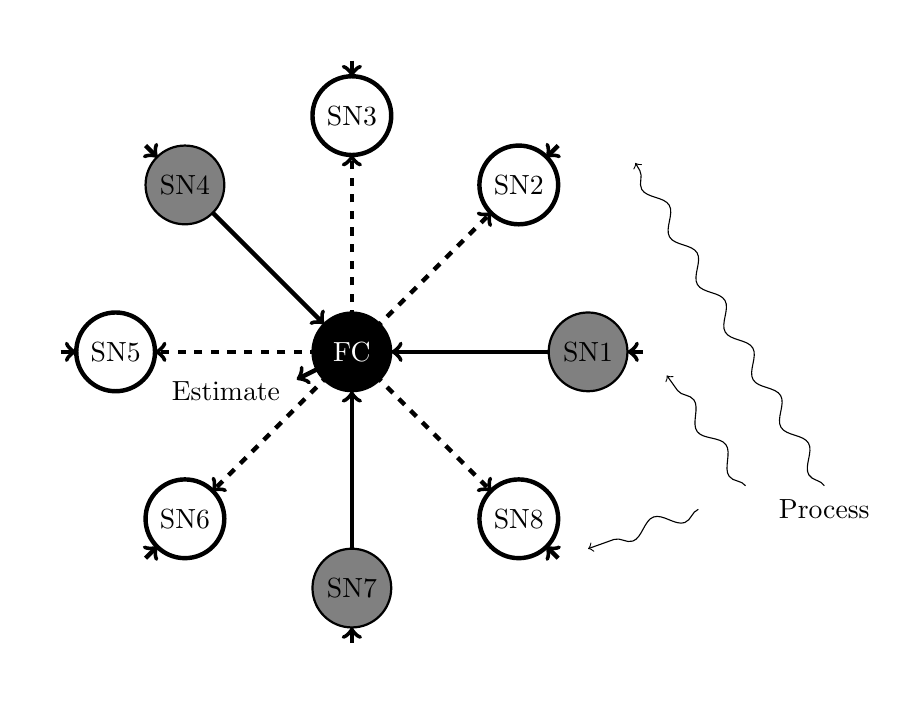
\begin{tikzpicture}
\draw [ultra thick, ->] (0,0) -- (-0.7,-0.35);
\node at (-1.6,-.5) {Estimate };
\draw [ultra thick, ->] (3,0) -- (0+0.5,0);
\draw [ultra thick, ->] (-2.12,2.12) -- (0-0.3535,0+0.3535);
\draw [ultra thick, ->] (0,-3) -- (0,0-0.5);
\node at (6,-2) {Process };
\draw [fill=black,draw=black,thick,text=white] (0,0) circle [radius=0.5];
\draw [fill=gray,draw=black,thick,text=white] (3,0) circle [radius=0.5];
\node at (3,0) {SN1};
\node at (4,0) {};
\draw [ultra thick, ->] (3.7,0) -- (3.5,0);
\def\x{3.5}
\def\y{0.35}
\draw [fill=white, ultra thick] (2.12,2.12) circle [radius=0.5];
\node at (2.12,2.12) {SN2};
\node at (2.83+0.2,2.83-0.2) {};
\draw [ultra thick,dashed, ->] (0,0) -- (2.47-0.7,2.47-0.7);
\draw [ultra thick, ->] (2.62,2.62) -- (2.47,2.47);
\def\x{2.12+0.6}
\def\y{2.12-0.25}
\draw [fill=white, ultra thick] (0,3) circle [radius=0.5];
\node at (0,3) {SN3};
\node at (0,4) {};
\draw [ultra thick,dashed, ->] (0,0) -- (0,2.5);
\draw [ultra thick, ->] (0,3.7) -- (0,3.5);
\def\x{0.6}
\def\y{3-0.25}
\draw [fill=gray,draw=black,thick,text=white] (-2.12,2.12) circle [radius=0.5];
\node at (-2.12,2.12) {SN4};
\node at (-2.83,2.83) {};
\draw [ultra thick, ->] (-2.62,2.62) -- (-2.47,2.47);
\def\x{-2.12-1.2-0.6}
\def\y{2.12-0.25}
\draw [fill=white, ultra thick] (-3,0) circle [radius=0.5];
\node at (-3,0) {SN5};
\node[above] at (-1.5,0) {};
\node at (-4,0) {};
\draw [ultra thick,dashed, ->] (0,0) -- (-2.5,0);
\draw [ultra thick, ->] (-3.7,0) -- (-3.5,0);
\def\x{-3.5-1.2}
\def\y{0.35}
\draw [fill=white, ultra thick] (-2.12,-2.12) circle [radius=0.5];
\node at (-2.12,-2.12) {SN6};
\node at (-2.83-0.2,-2.83+0.2) {};
\draw [ultra thick,dashed, ->] (0,0) -- (-2.47+0.7,-2.47+0.7);
\draw [ultra thick, ->] (-2.62,-2.62) -- (-2.47,-2.47);
\def\x{-2.12-1.2-0.6}
\def\y{-2.12-0.25}
\draw [fill=gray,draw=black,thick,text=white] (0,-3) circle [radius=0.5];
\node at (0,-3) {SN7};
\node at (0,-4) {};
\draw [ultra thick, ->] (0,-3.7) -- (0,-3.5);
\def\x{0-1.2-0.6}
\def\y{-3-0.25}
\draw [fill=white, ultra thick] (2.12,-2.12) circle [radius=0.5];
\node at (2.12,-2.12) {SN8};
\node at (2.83,-2.83) {};
\draw [ultra thick,dashed, ->] (0,0) -- (2.47-0.7,-2.47+0.7);
\draw [ultra thick, ->] (2.62,-2.62) -- (2.47,-2.47);
\def\x{2.12+0.6}
\def\y{-2.12-0.25}
\node [text=white] at (0,0) {FC};
\draw[->,decorate, decoration={snake, segment length=7mm, amplitude=1mm}] (5,-1.7) -- (4,-0.3);
\draw[->,decorate, decoration={snake, segment length=7mm, amplitude=1mm}] (4.4,-2) -- (3,-2.5);
\draw[->,decorate, decoration={snake, segment length=7mm, amplitude=1mm}] (6,-1.7) -- (3.6,2.4);
\end{tikzpicture}}
\vspace{-3mm}
\caption{A WSN for distributed estimation, with FC quality feedback.
Each SN decides to either remain idle with cost  or to collect and transmit to the FC the measurement  of  with local measurement SNR  and cost . The shared wireless channel results in collisions and packet losses. The FC, 
based on the measurements received, computes an MMSE estimate of , , and broadcasts the instruction  based on the estimation quality 
achieved,
which is used by the SNs to adjust their sensing-transmission parameters for the next slot.}\label{fig:WSN}
\vspace{-5mm}
\end{figure}

 This paper is organized as follows.
  In Sec.~\ref{probform}, we motivate our approach and summarize the main results.
  In Sec.~\ref{sysmo}, we present the system model and the optimization problem.
 In Sec.~\ref{analysis}, we present
 the analysis of the coordinated and decentralized schemes.
In Sec.~\ref{numres}, we provide numerical results.
In Sec.~\ref{conclusions}, we conclude the paper.
The analytical proofs are provided in the Appendix.
\vspace{-0.3cm}
\section{Motivation}
\label{probform}
 Consider a WSN, depicted in Fig.~\ref{fig:WSN}, with one FC, whose goal
 is to track a \emph{stationary Markov} process ,
 based on measurements collected  by  nearby SNs.
 The probability density function (if  is continuous, or probability mass function, if  is discrete) of  given  is denoted as 
 . In this paper, we consider the  scalar linear Gaussian state space model

where  is the slot index,
  is the \emph{time-correlation parameter}  and ,
 so that .
 This model arises, for instance, in temperature tracking applications, where  represents the temperature fluctuations around its mean \cite{Tandeo}.
 We denote the statistical power of  as ,
 and assume  , since any other value can be obtained by scaling.
 
Each SN incurs the transmission cost  to report its measurement to the FC.
   The  SNs share 
 a set of  orthogonal single-hop wireless channels to report their measurements to the FC.
 We employ the collision channel model, \emph{i.e.},
 the transmission on a given channel is successful if and only if one SN transmits in that channel. 
 This model is commonly employed in the analysis of multi-access communication schemes,
and lends itself to analysis.\footnote{Other channel models can be accommodated by defining, more generally, a probability mass function (PMF) , where
  and  are the number of SNs that transmit and of packets successfully received at the FC, respectively.}
 
Referring to the model (\ref{markovstate}),
 assume for simplicity 
 and that each SN measures  noiselessly (the noisy case with  is considered in the rest of the paper).
   Let  be the \emph{transmission outcome} for SN , \emph{i.e.},  if and only if its transmission is successful. 
    Then, if at least one measurement is collected at the FC, \emph{i.e.}, ,
 the MSE is . On the other hand, if no measurements are successfully received, \emph{i.e.}, , then
 is estimated via prediction. Therefore, if the transmission has been successful in slot , for some ,
so that  is perfectly known at the FC,
 but transmission failures or no transmission attempts occurred in slots , then  is estimated as  and
 the MSE at the end of slot  is .
 Due to the decentralized sensing-transmission decision of the SNs and the
  shared wireless channel, which may result in collisions among SNs, random and unpredictable fluctuations in the transmission outcome  may occur at the FC,
  so that the MSE evolves randomly over time. In order to control the uncertainty and system dynamics introduced by these cross-layer factors, we thus propose a
  feedback-based adaptive  scheme where
 the SNs adapt their activation strategy over time, \emph{i.e.}, whether to sense-transmit their measurement with cost  (denoted as ) or remain idle 
 with no cost (denoted as ), based on \emph{quality feedback} from the FC, captured by the state variable .
 The goal is to design the activation policy so as to minimize the expected MSE

 at the FC,\footnote{The slot index  is removed for simplicity to denote steady-state regime.}
under SN sensing-transmission cost constraints, .
We consider the following schemes.
\vspace{-3mm}
\subsection{Coordinated scheme}
\label{coordscheme}
 In this scheme, the FC centrally schedules the activation  of  each SN.
One design approach to optimize the MSE
is to maximize the number of measurements collected at the FC in each slot, under the cost constraint for each SN.
This is denoted as \emph{max aggregate SNR scheme} (MAX-SNR) in the rest of the paper.
If , the optimal strategy dictates to activate randomly one and only one SN in each slot,
resulting in a successful transmission, hence the MSE is  in each slot (Theorem \ref{thm1}). We thus have
 , , hence
 a \emph{non-adaptive} scheme is optimal in this case.
 \vspace{-3mm}
 \subsection{Decentralized scheme}
 \label{distscheme}
\noindent  Unfortunately, the coordinated scheme is not scalable to large WSNs,
 due to the centralized scheduling performed by the FC.
 Therefore, a decentralized approach, where the SNs make local decisions, leveraging only local information
 and minimal feedback information, is more practical.
 We thus devise
a decentralized scheme, where each SN activates with common probability  in slot .
 Following the same design principle of optimizing the expected number of measurements collected at the FC (MAX-SNR scheme),
we define a  \emph{non-adaptive} (NA) scheme where each
 SN activates with probability  in each slot, where we have defined the normalized transmission probability per channel .
In this case,  is a Markov chain.
Using the \emph{large network approximation}  with fixed ,
its transition probabilities are
,
 ,
 and the steady-state probability of  is given by   .
 By averaging over ,
 the average SN cost and MSE
 are
 
 
 \begin{table*}[t]

\caption{Main system parameters}
\vspace{-5mm}
\label{tab1}
\begin{center}
\footnotesize
\scalebox{0.88}{
\begin{tabular}{|c| l | c | l | c | l | c | l |}
\hline\T\B & random process to be tracked
&
& local ambient SNR
 &
& measurement of SN  in slot 
&
& accuracy state with 
 s.s.d. 
  \\\hline\T\B 
  & time-correlation parameter
&& local measurement SNR
&& activation of SN , slot 
&& channel ID for SN , slot 
\\\hline\T\B
 & aggregate SNR at FC
& & sensing cost
& & transmission cost
 && \# channels available, 
 \\\hline\T\B
 & prior variance 
& & posterior variance 
& & SN activation  probability 
&  & \# of SNs, 
\\\hline\T\B 
& normalized unitary sensing cost &
 & average MSE
&
 & 
\multicolumn{3}{l|}{
average sensing-transmission cost of SN 
}
\\
\hline
\end{tabular}
}
\end{center}
\vspace{-5mm}
\end{table*}

 
 Unfortunately, this design approach
 fails to achieve good performance in general,
since the decentralized SN activation and the collisions among SNs result in
random fluctuations in the number of measurements collected at the FC (which may be zero in case of collisions),
hence high uncertainty and poor MSE performance.
In order to control the uncertainty in the system, we propose an adaptive scheme
   where the activation probability  is adapted over time by the FC, based on the current quality
  state . Such adaptive policy is denoted as .
    The value of the activation probability  is broadcasted by the FC at the beginning of each slot.
    In particular, consider the myopic policy (MP), which 
   determines  in state  so as to 
    optimize a trade-off between the instantaneous 
    expected MSE and the cost for each SN,
    
    where  captures the desired trade-off,  is the probability that 
    no measurements are received at the FC, and  is the corresponding MSE achieved.
    The solution to this optimization problem is studied in Part II, and is given by
     if  ,
    otherwise it is the unique  solution of
     (see  \cite[Corollary~2]{MichelusiP2}).    
    Using the bound  in (\ref{MP}),
    we obtain the approximate MP (AMP), upper bound to ,
    
The AMP
     is an increasing function of , 
    \emph{i.e.}, the higher the uncertainty (the larger ), the higher the activation probability,
    which approaches  for .
\emph{Hence, AMP has the desirable property that,
the higher the uncertainty in the current estimate, the more the SNs are 
incentivized to activate, at higher cost, in order to estimate  accurately at the FC.}
Under AMP, we have
    
so that  the average SN cost and MSE
 are given by
 
 By varying  in (\ref{NA}),  in (\ref{AMP}), we obtain
  the cost-MSE  trade-off depicted in Fig.~\ref{TOYEX},
 which shows that AMP reduces the sensing-transmission cost for each SN by 30\% with respect to NA.
 Therefore,
  adaptation
 to the quality state yields performance gains in the cost-MSE trade-off and 
 effectively copes with the uncertainty introduced by the network and cross-layer components.
 
 \begin{figure}[t]
\centering
\includegraphics[width = .8\linewidth,trim = 10mm 4mm 10mm 9mm,clip=true]{figexample_c}
\vspace{-3mm}
\caption{Trade-off between network cost and MSE. , .}\label{TOYEX}
\vspace{-5mm}
\end{figure}


In the next sections, we will extend the analysis to the more general case ,
where the SNs collect noisy measurements of , whose quality is affected by an internal \emph{accuracy state} evolving as a Markov chain,
and by control performed by each SN.
In Theorem~\ref{thm1},
we will show that,
in the coordinated scheme,
 the MAX-SNR scheme, which maximizes the 
expected aggregate SNR collected at the FC in each slot under the SN cost constraint,
is optimal in the \emph{best}-  scenario, where
all SNs have deterministically the best accuracy state,
under some conditions on the maximum cost for each SN, .
In Theorem~\ref{thm2}, we will show that this strategy is near-optimal for \emph{large networks} in the \emph{Markov}- scenario,
where the accuracy state of each SN follows a Markov chain.
For the decentralized scheme, we derive structural properties
and exploit the large network approximation to design a DP algorithm with lower complexity. 
In Part II, we will further investigate the design of myopic policies for this more general setting,
for both the coordinated and decentralized schemes.

 \begin{remark}
This framework and the following analysis can also be applied  to other time-correlated signals, \emph{e.g.}, the two state Markov chain
 
 where  denotes the sum modulo 2,
  and  has distribution .
 This model  arises, for instance, in spectrum sensing applications \cite{MicheISIT},
 where  denotes the channel occupancy state ( if idle,  if busy).
In this case, the quality feedback is captured by the log-likelihood ratio ,
 reflecting the current detection accuracy, and the expected MSE can be replaced with the expected detection error probability.
 
The model (\ref{markovstate}) can also be extended to the multi-dimensional case, \emph{e.g.},
 in target tracking applications where the vector  represents the position and speed in slot .
 In this case,  is replaced by a proper matrix \cite{Xiao}, and the feedback quality is represented by the error covariance matrix (or by its trace, for
 dimensionality reduction purposes).
 \end{remark}
\section{System Model and Optimization Problem}
\label{sysmo}
 In this section, we present the system model. The main parameters are listed in Table \ref{tab1}.
Time is slotted and all SNs are assumed to be perfectly synchronized.\footnote{Note, however, that 
we also presume random access, which allows for some robustness against imperfect synchronization \cite{Gaudenzi}.}
 Each slot includes three~phases:
 \begin{enumerate}
 \item \emph{FC instruction} , broadcasted by the FC (Sec.~\ref{FCinstruct});
 \item \emph{Sensing and transmission to FC}: given , each SN selects its
 sensing-transmission action (Sec. \ref{ph2});
 \item \emph{Estimation at FC}: given the measurements collected, the FC estimates  via Kalman filtering (Sec.~\ref{P3}).
 \end{enumerate}
 \vspace{-5mm}
\subsection{Sensing and transmission to FC}
 \label{ph2}
\noindent  Each SN, at the beginning of slot , given the instruction  broadcasted by the FC,
  selects (possibly, in a randomized fashion) 
  the sensing-transmission parameters , 
 where  is the \emph{activation} decision of SN ,
  is the \emph{local measurement SNR} specified below, and  is the \emph{channel index}.
 If , SN  remains idle, hence  (no measurement collected) and  (no channel selected).
On the other hand, if , then  and
 the measurement of  collected by SN  is given by

where  is the \emph{ambient noise},
and  is the \emph{measurement noise} introduced by the sensing apparatus,
independent of each other, over time and across SNs,
   is the  \emph{local ambient SNR}, and  is the
   \emph{local measurement SNR}, controlled by the th SN, resulting in the sensing cost , for some .
 Note that this assumption is practical. For instance,
 SN  may compute an average from a controlled number  of independent measurements, each with
fixed ambient noise and i.i.d. measurement noise with  variance 
 and cost ,
 resulting in the local measurement SNR  and in the overall
 sensing cost .

   
We assume that
   a fixed quantization scheme is employed, \emph{i.e.}, a fixed number of bits is transmitted to the FC,\footnote{Therefore, 
   the ambient SNR  and noise  can also be interpreted, respectively, as the quantization SNR floor and the Gaussian approximation of the quantization error.}
and that each SN is unaware of its own distance to the FC
and it does not employ power adaptation, but it
 transmits with constant power, so as to provide a given coverage requirement,
resulting in the overall transmission cost , common to all SNs.
 The FC is assumed to be within the coverage area 
of each SN. A varying  can be easily incorporated with increased book-keeping.
We define the \emph{normalized unitary sensing cost} .
No cost is incurred if the SN remains idle.
The overall sensing-transmission cost
is thus .
We define the \emph{sample average sensing-transmission cost for SN } over a time horizon of length  as


The \emph{accuracy state} , taking values in the finite set , models the ability of SN  to accurately measure .
We model it as a Markov chain with transition probability  
and steady-state distribution ,
i.i.d. across SNs, and we let .
{Such a model arises, \emph{e.g.}, in a target tracking application, where the power of the received signal diminishes with the distance, which 
evolves following Markov dynamics as a function of the relative motion of the SN and the target  \cite{Xiao}.
The Markov assumption on  is used for analytical tractability, but the following analysis requires only the existence of
the steady-state distribution , and therefore it applies to non-Markov dynamics as well.}
In practice,  varies slowly over time, \emph{e.g.}, as a function of the SN position with respect to the
source of the process , and therefore it can be tracked accurately
 from the sample mean and sample variance estimates of the measurement noise. 
  We denote the best accuracy state as ,
and, without loss of generality, we assume  and .
 We denote the general scenario where  follows a Markov chain as \emph{Markov-} scenario,
and the special cases where ,  deterministically 
and  is i.i.d. over time as \emph{best-} and \emph{i.i.d.-} scenarios, respectively.
\vspace{-3mm}
\begin{remark}
\label{rem22}
 Note that the local accuracy state may vary significantly over both time and space, yielding instantaneous \emph{asymmetries} in the WSN. Typically, design of 
 asymmetric systems suffers from the curse of dimensionality. Herein, we assume that \emph{statistical symmetry} holds, in the sense that, in the long term, the SNs have the same statistical view of the system, despite the local temporal and spatial fluctuations of the state. 
 As a consequence, we assume \emph{policy symmetry}, \emph{i.e.}, all SNs employ the same policy to map
 their local state to a sensing-transmission action, thus significantly reducing the policy space and the optimization complexity.
 \end{remark}


\subsection{MMSE estimator at the FC via Kalman filtering}
\label{P3}
\noindent The weighted average measurement
   
   is a sufficient statistic for ,
   where  is the \emph{local SNR} for SN , defined as
   
    Given the transmission outcome and ,
    is a Gaussian random variable with mean  and variance
   ,
where we have defined the \emph{aggregate SNR} collected at the FC as



 Let  and  be the posterior mean (\emph{i.e.}, the MMSE estimate)
and variance of  at the FC at the end of slot ,
\emph{i.e.},  is the belief of  at the FC.
 Before collecting the measurements from the SNs in slot ,
 using~(\ref{markovstate}),
 the belief of  is ,
 where  is the \emph{prior variance} of ,
defined recursively as

Then, upon collecting the weighted average measurement  (\ref{bari})
 with aggregate SNR ,\footnote{We assume that each active SN, in addition to , also provides to the FC the value of 
and , which is employed in the Kalman filter.}
the FC updates the \emph{posterior variance}  and  mean  of  as

The function  in (\ref{nu}) determines  the prior variance of , given the posterior variance of ,
whereas  in (\ref{nu2}) determines the posterior variance of , given its prior variance ,
as a function of the aggregate SNR  collected at the FC.
The MSE in slot  is thus

We define recursively 
and, for ,

where  is the aggregate SNR sequence collected at the FC
from slot  to slot . Then,
we can write .
We define the \emph{sample average MSE} under  over a time horizon of length  as

Note that the prior and posterior variances  and  take value between ,
where the extreme values  and  correspond, respectively, to
 minimum ( perfectly known) and maximum ( is completely unknown) uncertainty.
Therefore, , and the system is stable.
\vspace{-4mm}
\subsection{FC instruction policy}
\label{FCinstruct}
\begin{table}[t]
\caption{FC instruction  policy}
\vspace{-8mm}
\label{tabins}
\begin{center}
\footnotesize
\scalebox{0.83}{
\begin{tabular}{|c| c | c | c |}
\hline\T\B 
\multirow{2}{*}{\em Scheme} & \multirow{2}{*}{\em Activity }  & \em Local measurement & \multirow{2}{*}{\em Channel ID }\\
&  &\em SNR  & 
\\\hline\T\B 
{\bf Coordinated}    & Centralized,  FC & Centralized,  FC & Centralized,  FC
\\\hline\T\B 
\multirow{2}{*}{{\bf Decentralized}} & Local, w.p.  & Local,  & \multirow{2}{*}{Local, random}
\\
 &  given by FC &   given by FC  &
\\
\hline
\end{tabular}
}
\end{center}
\vspace{-9mm}
\end{table}

\noindent At the beginning of  slot ,
the FC broadcasts an
\emph{instruction} , which, together with the local accuracy state ,
is used by SN  to select  as in Sec. \ref{ph2}. We consider the following schemes, summarized in Table \ref{tabins}:
\subsubsection{Coordinated scheme}
  In the coordinated scheme, given  and , the FC schedules the sensing-transmission action  of  each SN,  so that .
Note that each SN is required to report its accuracy state to the FC, whenever its value changes,
  so that  is perfectly known at the FC at the beginning of slot .
  Letting  be the belief of  at the FC, we have that
  ,
  where  is the indicator function. 
  In Sec.~\ref{commover}, we will analyze the cost of communication overhead to keep such state information at the FC.
The value  is selected according to some (possibly, non-stationary) \emph{instruction policy}
 .
\subsubsection{Decentralized scheme}
 In the decentralized scheme, the FC specifies ,
  where  and 
  are, respectively,
the activation probability and 
the local measurement SNR functions  employed by each SN to select their sensing-transmission strategy in a decentralized manner, as a function of the local accuracy state .
Therefore,  takes value in the set ,
and is generated according to some (possibly, non-stationary) policy , where

is the belief state of the accuracy state vector , given the history of observations collected up to time  at the FC, . 
Given 

and the local accuracy state ,
 SN  chooses its action 
as  with probability ,
 otherwise; if , then
 and  is chosen uniformly from the set of  channels 
{(if , then ).}
Due to the randomized channel accesses, this scheme may result in collisions among SNs.
\vspace{-3mm}
\begin{remark}
\label{PMF}
The choice of a randomized uniform channel access decision by the SNs is due to their decentralized operation and 
lack of coordination between them. However, other channel access schemes can be accommodated by defining, more generally, the PMF .
\end{remark}


For both schemes, given the instruction policy ,
the sequence  is a Markov chain.
In fact, the instruction  is chosen according to
.
Each SN decides its action  based on
 and , so that the aggregate SNR collected at the FC, , is a random variable
 which only depends on  and  and is independent of the past.
Finally, given , from (\ref{nu}) and (\ref{nu2}) the next prior variance state is
, and 
only depends on , whose distribution is , and is independent of other past events, so that the Markov property holds.
For the decentralized scheme, the next belief state  can be computed as a function of 
 the measurements collected in slot , and channel collisions.
On the other hand, for the coordinated scheme,  is a function of ,
whose value is fed back by the SNs.
\vspace{-3mm}
\begin{remark}
\label{remiid}
If , the process  is i.i.d., hence . In this case, both schemes do not adapt to the quality feedback , but only to the belief on the accuracy state 
. On the other hand, in the time-correlated case , adaptation to the quality state  may be necessary to achieve optimality, \emph{e.g.}, by instructing the SNs to remain idle if the quality of the estimate is good enough.
\end{remark}
\vspace{-8mm}
\subsection{Performance metrics and optimization problem}
\label{sec:optprob}
\noindent Given the initial value of the prior variance , the initial distribution , and the instruction policy ,
we define the average MSE and sensing-transmission cost of SN   over a finite horizon of length 
as 
{
where  is the sample average MSE given by (\ref{RT}),
and 
is the \emph{sample average sensing-transmission cost for SN }, given by (\ref{ctn})}.
The expectation is computed with respect to the activation, local measurement SNR, accuracy state and medium access processes 
, induced by policy .
The goal is to determine  such that

where  is the maximum network cost constraint.
Alternatively,
we consider the Lagrangian formulation

where  is the Lagrange multiplier, which trades off MSE and sensing-transmission cost.
 In particular, we are interested in the infinite horizon   (average long-term)
 and ,
 so that we will drop the dependence  on  and  in the following treatment, whenever possible.
 By varying  in (\ref{optprob}) (respectively,  in (\ref{optproblag})),
we obtain different operational cost-MSE points .
\vspace{-3mm}
\begin{remark}
\label{remoutage}
Note that the posterior variance process  may exhibit significant fluctuations over time, which may be undesirable. 
These fluctuations can be reduced by imposing a constraint on the frequency that a given MSE threshold  is overcome,
defined by the \emph{outage} event , and by the time average expected outage

The constraint 
can then be added to the optimization problem (\ref{optprob}), or the Lagrangian term 
to  (\ref{optproblag}).
The following DP algorithm (\ref{DPgen}) can be straightforwardly extended to this case. Its analysis is left for future~work.
\end{remark}
\vspace{-0.3cm}
\section{Analysis}
\label{analysis}
\noindent For the finite horizon , for both the coordinated and decentralized schemes, the optimal instruction policy ,
which is the solution of (\ref{optproblag}), can be found
via DP \cite{Bertsekas2005}, by solving recursively, backward in time from  to ,

where  and .
The minimizer is the optimal instruction policy  in slot ,
and  yields the optimal cost function for the Lagrangian problem (\ref{optproblag}).
The infinite horizon scenario  can be approximated by choosing  sufficiently large.
In general, (\ref{DPgen}) has high complexity, due to the large action space, non-convex nature, and the dependence on the accuracy state belief 
.
In particular, in the coordinated scheme, the optimization is over the joint action 
of each SN, as a function of  and  and time .
On the other hand, in the decentralized scheme, the optimization is over functions
 and .
To overcome these dimensionality issues,
in Secs.~\ref{centr} and \ref{deccentr} we derive structural properties of the optimal policy and of the cost function by exploiting the \emph{statistical symmetry}
 and the \emph{large network} approximation ,
which enable a more efficient solution of (\ref{DPgen}). In Part II, we will further reduce the complexity by proposing
 near-optimal myopic policies.
Theorem \ref{lowbound} lower bounds the optimal MSE under any scheme.
\begin{thm}
\label{lowbound}
If , we have
,
where

\end{thm}
\noindent\emph{Proof:}
The proof follows from the fact that  is a convex function of  (Prop.~\ref{propV} in App.~\ref{appprop}),
hence . 
Letting  be the average aggregate SNR, we have 
,
where  is defined in (\ref{RTstar}). Since  is a decreasing function of  (Theorem~\ref{thm3} in App.~\ref{appprop}) and 
 as a result of the optimization in (\ref{maxagg}),
we also have . Finally, in the limit , using Corollary~\ref{corollary} in App.~\ref{appprop},
we obtain , proving the theorem.\hfill\QED


The policy solving the optimization problem (\ref{maxagg}) is denoted as the \emph{max aggregate SNR scheme} (MAX-SNR). In each slot, it maximizes the expected 
aggregate SNR collected at the FC, under the cost constraint for the SNs.
MAX-SNR is non-adaptive, since it is independent of .
The lower bound in Theorem \ref{lowbound} can be achieved only if the aggregate SNR  is collected deterministically in each slot
 (Corollary~\ref{corollary} in App.~\ref{appprop}).
However, this lower bound is, in general, not achievable, 
since the cross-layer factors introduce uncertainties and random fluctuations of the aggregate SNR  around its mean, thus
degrading the MSE performance. Hence, MAX-SNR may achieve poor performance in general, as shown in Sec. \ref{numres}.
We now analyze both schemes.
\vspace{-3mm}
\subsection{Analysis  of Coordinated scheme}
\label{centr}
\noindent In the coordinated scheme, collisions can be avoided by scheduling at most one SN to transmit in each channel.
Without loss of optimality, the SNs are scheduled to transmit, in order, in
the channels with ID . Therefore,
if , we let . This channel scheduling is optimal, since the  orthogonal channels are symmetric and interchangeable.
We proceed as follows. We first derive structural properties of the optimal policy and of the DP
algorithm by exploiting the statistical symmetry of the WSN for the \emph{best-} scenario, yielding a lower bound to the MSE
achievable under the  \emph{Markov-} scenario.
Based on that, we then
design low-complexity policies for the
 \emph{Markov-} scenario, 
 which are shown to be near-optimal for large WSNs.
\subsubsection{\emph{Best-} scenario}
In this case, the belief  is constant and  can be neglected.
 Prop. \ref{optsymm} states the optimality of \emph{policy symmetry}, \emph{i.e.}, due to the statistical symmetry of the WSN,
it is optimal for the FC to schedule actions \emph{uniformly} randomly  across SNs.
In other words, the SNs incur the same sensing-transmission cost
and have the same sensing capabilities, hence there is no preference of one SN over another.
Let

be an ordered subset of instructions. We have that any instruction  can be obtained
by permutation of some . Additionally, let  be the subset of instructions in
 obtained by permutation of the entries of ,
so that . 
\begin{propos}
\label{optsymm}
In the \emph{best-} scenario,
one optimal instruction policy  for (\ref{optprob}) or (\ref{optproblag}) satisfies, ,

\end{propos}
\noindent\emph{Proof:}
See App.~\ref{Proofoptsymm}.
\hfill\QED

\noindent 
We denote an instruction policy satisfying the hypothesis of Prop.~\ref{optsymm}
as a \emph{symmetric instruction policy}. Such a policy is symmetric with respect to the SN scheduling, and induces
 the same expected cost for each SN, so that the superscript  in (\ref{CSN}) can be neglected.
To generate a symmetric instruction policy,
the FC first selects
 one ordered instruction  from the lower-dimensional set , and then
  assigns, in order, each component of  to a random SN, until
all of them have been scheduled. 
The following proposition
  demonstrates the optimality of
allocating the same local measurement SNR to all active SNs.
\begin{propos}
\label{lem2}
In the \emph{best-} scenario,
the optimal  allocates  for all  such that .
\end{propos}
\noindent\emph{Proof:}
See App.~\ref{Proofoptsymm}.
\hfill\QED

\noindent
This result follows from the concavity of the aggregate SNR with respect to the SNR allocation of the SNs.
Under the resource constraints, it is thus optimal for the SNs to employ the same SNR, in order to maximize the aggregate SNR collected at the FC.
 From Props. \ref{optsymm} and \ref{lem2}, it follows that, in the \emph{best-} scenario, it is sufficient for the FC to choose, in each slot ,
the number of SNs to activate , and their common local measurement SNR . The  active SNs
are then chosen uniformly from the set of SNs.
For a given pair ,
the aggregate SNR collected at the FC is thus .
The MSE performance is governed by the aggregate SNR  collected at the FC. Since the FC 
can control , we can optimize these two quantities to minimize the sensing-transmission cost
in order to collect the target aggregate SNR  at the FC,
denoted as ,
 yielding the following proposition.
\begin{propos}
\label{lem3}
Let  be the target aggregate SNR collected at the FC.
In the \emph{best-} scenario,
if , then  and .
Otherwise (), let

then 
and , where  is the unique value such that .
\end{propos}
\noindent\emph{Proof:}
See App.~\ref{Proofoptsymm}.
\hfill\QED

\noindent From Prop.~\ref{lem3}, it follows that it is sufficient for the FC to determine, in each slot ,
the target aggregate SNR . The number of SNs activated is then given by ,
 and the common local measurement SNR is .
  Note that  is an increasing function of , implying that an increasing number of SNs need to be activated 
as the aggregate SNR requirement  increases.
Moreover,  is an increasing function of  
and decreasing function of the normalized unitary sensing cost , so that, as  grows or  diminishes,
less SNs need to be activated.
In fact,  determines the error floor in the measurement collected by each SN. 
Therefore, as  increases and the ambient noise becomes less relevant, it is sufficient to activate 
a smaller number of SNs with higher SNR, in order to reduce the transmission cost.
Similarly, as  grows, the
transmission cost becomes less and less relevant with respect to the sensing cost, hence
more SNs can be activated.
We thus obtain:

\noindent {\bf COORD-DP: DP algorithm for the coordinated scheme, \emph{best-} scenario.}
 For , solve, ,
  
where . The optimizer, , is the optimal aggregate SNR collected at the FC in slot .
\hfill\QED

Note that, by exploiting the statistical symmetry of the WSN, we have enabled a significant complexity reduction with respect to 
 (\ref{DPgen}), since the optimization is only over the aggregate SNR sequence, rather than the joint action  of each SN.
 
The next theorem characterizes regimes of  where the optimal policy is the MAX-SNR scheme.
\begin{thm}
 \label{thm1}
In the \emph{best-} scenario with ,
\ii) if ,
  is the MAX-SNR scheme, 
with , ;
\
\!\!\nonumber \left\{
\begin{array}{l}
\!\!\!\!A_{r(m;\boldsymbol{\gamma}_k),k}\!=\!1,\ \!\!S_{M,r(m;\boldsymbol{\gamma}_k),k}\!=\!S_{M,k}^*,\forall m\!=\!1,2,\!\dots\!,\!t_k^*,
\\
\!\!\!\!A_{r(m;\boldsymbol{\gamma}_k),k}\!=\!0,\ \forall m>t_k^*.\hfill\QED
\end{array}
\right.

&
\!\!\!0\!\leq\!\bar M_{\delta^*}\!\!-\!\bar M_{\delta^*}^{\gamma_{\max}}
\!\!\leq\!
\frac{1}{1\!-\!\alpha}\!\exp\!\left\{\!\!-\frac{\left(N_S\pi_{\gamma}(\gamma_{\max})\!-\!B\!+\!1\right)^2}{2N_S\pi_{\gamma}(\gamma_{\max})}\!\!\right\}\!.\!\!\!
\label{inex}

\label{DP}
&\bar W^{T-k}(V_{k},\pi_{\boldsymbol\gamma,k})
=
\min_{\!\!\!\!\!\!\!(q,S_M):\Gamma\mapsto[0,1]\times[0,\infty)\!\!\!\!\!\!\!}
\mathbb E\left[\left.\hat \nu\left(V_{k},\Lambda_k\right)\right|q,S_M\right]
\nonumber\\&
+
\frac{\lambda}{c_{\mathrm{TX}}} \!\!\!\sum_{\boldsymbol\gamma\in\Gamma^{N_S}}\pi_{\boldsymbol\gamma,k}(\boldsymbol\gamma)\sum_{n=1}^{N_S}q(\gamma_n) c_{SN}(1,S_{M}(\gamma_n))
\nonumber
\\&
+
\mathbb E\left[\left.
\bar W^{T-k-1}\left(\nu\left(\hat \nu\left(V_{k},\Lambda_k\right)\right),\pi_{\boldsymbol\gamma,k+1}\right)\right|q,S_M\right],

p_R(r;q)\!\!=\!\!
\sum_{k=r}^{B}\!
\frac{(-1)^{k-r}N_S!}{(N_S-k)!}\!\!
\left(\begin{array}{c}\!\!\!\!B\!\!\!\!\\\!\!\!\!r\!\!\!\!\end{array}\right)\!\!
\left(\begin{array}{c}\!\!\!B-r\!\!\!\\\!\!\!k-r\!\!\!\end{array}\right)\!\!
\left(\frac{q}{B}\right)^{k}\!\!
\left(1\!-\!k\frac{q}{B}\right)^{\!\!N_S-k}\!\!\!\!\!\!\!.

  \label{DPzeta}
&\!\!\!\!\bar W^{T-k}(V_{k})
\!\!=\!\!\min_{\zeta,S_{M}}\!\sum_{r=0}^Bp_R(r;\zeta)\hat \nu\left(\!\!V_{k},r\frac{S_AS_M}{S_A\!\!+\!\!S_M}\!\right)
\!\!+\!\!\frac{\!\lambda\zeta\!}{\!c_{\mathrm{TX}}\!} c_{SN}(1,\!S_{M}\!)
\nonumber
\\&
\!+\!\sum_{r=0}^Bp_R(r;\zeta)
\bar W^{T-k-1}\left(\nu\left(\hat \nu\left(V_{k},r\frac{S_AS_M}{S_A+S_M}\right)\right)\right),

q_k(V_k,\gamma)=
\left\{
\begin{array}{ll}
1,&\gamma >\gamma_{\mathrm{th}},\\
\frac{\frac{B}{N_S}\zeta_k^{*}(V_k)-\sum_{\gamma>\gamma_{\mathrm{th}}}\pi_{\gamma}(\gamma)}{\pi_{\gamma}(\gamma_{\mathrm{th}})},
&
\gamma=\gamma_{\mathrm{th}},\\
0,&\gamma<\gamma_{\mathrm{th}},
\end{array}
\right.

(\zeta^*,S_M^*){=}\underset{\zeta,S_M}{\arg\max}\frac{\mathbb E[\left.R_k\right|\zeta]S_AS_M}{S_A+S_M}\ \text{s.t.}\ B\zeta(c_{\mathrm{TX}}+\phi S_M)\leq\epsilon,

\label{censrule}
\left|Y_{n,k}-\gamma_{n,k}\sqrt{\alpha}\hat X_{k-1}\right|<\tau\sqrt{\gamma_{n,k}^2V_k+S_A^{-1}+S_M^{-1}},

(q^*\!\!,\!S_M^*)\!=\!\!\!\!&\underset{q\in[0,1],S_M\geq 0}{\arg\max}\!\!\!\!qN_Se^{-\frac{qN_S}{B}}\!\!\frac{S_AS_M}{S_A\!+\!S_M},
\text{s.t. }qc_{\mathrm{TX}}\!+\!\phi S_M\!\!\leq\!\!\frac{\epsilon}{N_S}\!.

&\hat \delta_k(\mathbf D|V_{k})\!=\!\frac{1}{|\mathcal D(\mathbf D^{(O)})|}\!\sum_{\tilde{\mathbf D}\in \mathcal D(\mathbf D^{(O)})}\!\!\!\delta_k(\tilde{\mathbf D}|V_{k}),\ 
\forall \mathbf D\in \mathcal D(\mathbf D^{(O)}).

\label{sm}
\tilde S_{M}=
\frac{
\sum_{m=1}^{t}A_mS_{M,m}/(S_A+S_{M,m})
}
{
\sum_{m=1}^{t}A_m/(S_A+S_{M,m})
},

&
\mathbb E[c_{SN}(A_{n,k},S_{M,n,k})|\tilde{\mathbf D}^{(O)}]
=
\frac{t}{N_S}c_{SN}(1,\tilde S_{M})
\\&\nonumber
\leq
\frac{t}{N_S}c_{SN}\left(1,\frac{1}{t}\sum_{n=1}^{t}S_{M,n}\right)
=\mathbb E[c_{SN}(A_{n,k},S_{M,n,k})|{\mathbf D}^{(O)}],

\label{opwreter}
\!\!\!\bar\Lambda^*\!\!\!=\!\max_{p,S_M}\!\!\sum_{t=1}^B\!\!\frac{p(t)tS_AS_M\!(t)}{S_A+S_M(t)},\!
\text{s.t.}\!\!\sum_{t=1}^B\!\!p(t)t\!\left(c_{\mathrm{TX}}\!+\!\phi S_{M}\!(t)\right)\!\leq\!\epsilon.\!\!\!
&S_M^*(\cdot)\!=\!\arg\max_{S_M}\!\!\sum_{t=1}^Bp(t)t\!\left[\frac{S_AS_M(t)}{S_A+S_M(t)}-\mu\left(c_{\mathrm{TX}}+\phi S_{M}(t)\right)\right]\!.\!\!

&\bar\Lambda^*\!=\max_{\bar m\in [0,\min\{\epsilon/c_{\mathrm{TX}},B\}]}\frac{\bar mS_A(\epsilon-c_{\mathrm{TX}}\bar m)
}{\bar m\left(\phi S_A-c_{\mathrm{TX}}\right)+\epsilon
}.

\lim_{T\to\infty}R_T(1;\bar \Lambda\mathbf 1_{T+1})=\hat\nu^*(\bar \Lambda).

\hat V_{k+1}=\hat\nu(\nu(\hat V_{k}),\bar\Lambda)
<\hat\nu(\nu(\hat V_{k}),\hat\Lambda)=\hat V_{k},

\hat\nu^*(\bar\Lambda)=\hat\nu(\nu(\hat\nu^*(\bar\Lambda)),\bar\Lambda)<
\hat\nu(\nu(\hat V_k),\bar\Lambda)=\hat V_{k+1},

\sum_{k=\bar k}^{\bar k+J-1}\hat V_k=
\sum_{k=\bar k}^{\bar k+J-1}\hat\nu^{k-\bar k}(V_{\bar k};\Lambda_{\bar k}^{k,*}).

&\sum_{k=\bar k}^{\bar k+J-1}\hat V_k\leq\!\!\!\!
\sum_{k=\bar k}^{\bar k+J-1}\left[\hat V_k^*
+
\left.\frac{\mathrm d\hat\nu^{k-\bar k}(v;\Lambda_{\bar k}^{k,*})}{\mathrm d v}\right|_{v=V_{\bar k}^*}\!\!\!\!\!\!\!\!\!\!(V_{\bar k}-V_{\bar k}^*)\right]
\nonumber\\&
\leq
\sum_{k=\bar k}^{\bar k+J-1}\left[\hat V_k^*+\alpha^{k-\bar k+1}\right]
\leq
\hat V_{\bar k}^*+\frac{\alpha}{1-\alpha}+\sum_{k=\bar k+1}^{\bar k+J-1}\hat V_k^*.

&\sum_{k=0}^{T}\hat V_k\leq
(1-Q_0)\hat V_0^*
\!+\!\sum_{k=1}^{T}\!\left[
(1-Q_k)(1-Q_{k-1})\hat V_k^*+Q_k
\right]
\nonumber\\&
\!+\!Q_0\!+\!\sum_{k=1}^{T}\!(1\!-\!Q_k)Q_{k-1}\!\left(\hat V_{k}^*\!+\!\frac{\alpha}{1-\alpha}\right)
\!\!=
\!\!\sum_{k=0}^{T}\hat V_k^*
\!+Q_0(1\!-\!\hat V_0^*)
\nonumber\\&
\!\!+\!\!\sum_{k=1}^{T}\!
\left[
\frac{\alpha(1-Q_k)Q_{k-1}}{1-\alpha}
+Q_k(1-\hat V_k^*)
\right]
\!\leq\!
  \sum_{k=0}^{T}\!\left(\hat V_k^*+\frac{Q_k}{1-\alpha}\right)\!.

\mathcal Q\triangleq \mathbb P(Q_k=1)\!
=\!\sum_{i=0}^{B-1}\left(\begin{array}{c}\!\!\!N_S\!\!\!\\i\end{array}\right)\pi_{\gamma}(\gamma_{\max})^i
(1\!-\!\pi_{\gamma}(\gamma_{\max}))^{N_S-i},

&U(t,b)=\sum_{n=0,n\neq 1}^t\left(\begin{array}{c}t\\n\end{array}\right)U(t-n,b-1),

\nn
&U(t,b)\!=\!\!\!\!\!\!\!\!\!\!\sum_{k=0}^{\min\{t,b-1\}}\!\!\!\!\!\!\!\!(-1)^k\!\!
\left(\begin{array}{c}\!\!b\!\!\\\!\!k\!\!\end{array}\right)\!\!
\frac{t!}{(t-k)!}
(b-k)^{t-k}
\!+b!\chi(t=b)(-1)^b,
\\&
\text{hence }p_{R|T}(r|t)=\left(\begin{array}{c}B\\r\end{array}\right)\frac{t!}{(t-r)!}\frac{U(t-r,B-r)}{B^t},

p_R(r;q)=
\sum_{t=r}^{N_S}
\left(\begin{array}{c}\!\!\!\!N_S\!\!\!\!\\\!\!\!\!t\!\!\!\!\end{array}\right)
q^t(1-q)^{N_S-t}\left(\begin{array}{c}\!\!\!B\!\!\!\\\!\!\!r\!\!\!\end{array}\right)\frac{t!U(t-r,B-r)}{(t-r)!B^t},

\label{DPzeta2}
&f(\zeta)
\triangleq
-\sum_{r=1}^B\mathbb P(R_k\geq r|\zeta)
\\&
\times\left[\hat \nu\left(V_{k},(r-1)S_T\right)-\hat \nu\left(V_{k},rS_T\right)-(W(r-1)-W(r))\right],
\nonumber

\mathbf P_k=\left[
\begin{array}{cc}
\alpha & 1-\alpha
\\
\alpha\Lambda_k&1+(1-\alpha)\Lambda_k
\end{array}\right].

\label{derivSi}
&\frac{\mathrm d\hat\nu^k(V_0;\Lambda_0^{k})}{\mathrm d \Lambda_i}
=-\frac{1}{ D_k^2}
\mathbf X_{k}^T
\left[
\begin{array}{cc}
0 & 1
\\
-1&0
\end{array}\right]
\frac{\mathrm d\mathbf X_{k}}{\mathrm d\Lambda_i}
\\&\nonumber
=
\!-
\mathbf X_{k}^T
\left[
\begin{array}{cc}
0 & 1
\\
-1&0
\end{array}\right]
\mathbf P_{k:i+1}
\left[\begin{array}{c}0\\1\end{array}\right]
\frac{N_{i}}{ D_k^2}
=-\alpha^{k-i}\frac{N_i^2}{ D_k^2}<0,

 \mathbf H_{i,j}
\!\!=\!\!\frac{\!\mathrm d^2\hat\nu^k(V_0\!;\!\Lambda_0^{k})\!}{\mathrm d \Lambda_i\mathrm d \Lambda_j}
\!\!=\!\!
\frac{\!2N_i^2\alpha^{k-i}\!\!\!\!\!\!\!\!}{ D_k^3}[0,\!1]\frac{\mathrm d\mathbf X_k}{\mathrm d\Lambda_j}
\!\!=\!\!
\frac{\!2N_i^2\!N_{j}\alpha^{k-i}\!\!\!\!\!\!\!\!}{ D_k^3}
[0,\!1]\mathbf P_{k:j+1}\!\!
\left[\begin{array}{c}\!\!\!0\!\!\!\\\!\!\!1\!\!\!\end{array}\right]\!\!.

\label{f}
[\mathbf D^{-1}\mathbf H\mathbf D^{-1}]_{i,j}
=
\frac{2}{ D_k^3}
\frac{[0,1]\mathbf P_{k:j+1}[0,1]^T}
{N_j\alpha^{k-j}}\triangleq f_j.

[0,1]\mathbf P_{k:i+1}[0,1]^T
N_{i+1}
>
\alpha
[0,1]\mathbf P_{k:i+2}[0,1]^T
N_i,

&[0,1]\mathbf P_{k:i+2}
\left[\mathbf P_{i+1}[0,1]^T[\alpha,1-\alpha]
-[0,1]^T[\alpha,0]\right]
\mathbf X_i
\nonumber\\&
=
(1-\alpha)[0,1]\mathbf P_{k:i+2}
\mathbf P_{i+1}\mathbf X_i
=
(1-\alpha) D_k
>
0,

\label{derivV}
&\frac{\mathrm d\hat\nu^k(V_0;\Lambda_0^{k})}{\mathrm d V_0}
=
-\frac{1}{ D_k^2}
\mathbf X_{k}^T
\left[
\begin{array}{cc}
0 & 1
\\
-1&0
\end{array}\right]
\frac{\mathrm d\mathbf X_{k}}{\mathrm dV_0}
\\\nonumber
&=
-\frac{1}{ D_k^2}
[
V_0,1+V_0\Lambda_0
]
\mathbf P_{k:1}^T\!\!
\left[
\begin{array}{cc}
0 & 1
\\
-1&0
\end{array}\right]\!\!
\mathbf P_{k:1}\!\!
\left[
\begin{array}{c}
\!\!\!1\!\!\!\\\!\!\!\Lambda_0\!\!\!
\end{array}
\right]
\!=\!
\frac{\alpha^{k}}{ D_k^2}>0,

\frac{\mathrm d^2\hat\nu^k(V_0;\Lambda_0^{k})}{\mathrm d V_0^2}
\!\!=\!\!-\frac{2\alpha^{k}}{ D_k^3}[0,1]\frac{\mathrm d\mathbf X_{k}}{\mathrm dV_0}
\!=\!
-\frac{2\alpha^{k}}{D_k^3}[0,1]
\mathbf P_{k:1}\!\!
\left[
\begin{array}{c}
\!\!\!1\!\!\!\\\!\!\!\Lambda_0\!\!\!
\end{array}
\right]\!\!<\!\!0,

\label{RTstar}
\!\!\!\!R_T^*(\bar\Lambda)=\!\!\!\min_{\Lambda_0^T,\Lambda_k\geq 0,\forall k} R_T(1;\Lambda_0^{T}),
\ \text{s.t.}\ 
\frac{1}{T+1}\sum_{k=0}^T\Lambda_k=\bar\Lambda,

\Lambda_{0,m}^*\!\!\triangleq\!\!\frac{\sqrt{\frac{1-\alpha^{m+2}}{1-\alpha^{m+1}}}-1}{1-\alpha},\ 
\Lambda_{1,m}^*\!\!\triangleq\!\!\Lambda_{0,m}^*\left(\!\!1\!-\!\alpha\sqrt{\frac{1-\alpha^{m+1}}{1-\alpha^{m+2}}}\right)\!\!.

\label{cond}
\!\!\!\!\!\frac{\Lambda_{0,m}^*\!\!\!+\!(T\!-\!m\!-\!1)^+\!\Lambda_{1,m}^*}{T+1}\!\!\leq\!\!\bar \Lambda\!\!<\!\!\frac{\Lambda_{0,m-1}^*\!\!+\!(T\!-\!m)^+\!\Lambda_{1,m-1}^*}{T+1}.\!\!\!

&\Lambda_0^*=(T+1)\bar \Lambda\in [\Lambda_{0,m}^*,\Lambda_{0,m-1}^*),\ \Lambda_k^*=0,\ k>0;
\\&
\label{RT1}
R_T^*(\bar\Lambda)=1-\frac{1}{T+1}\frac{1-\alpha^{T+1}}{1-\alpha}\frac{(T+1)\bar \Lambda}{1+(T+1)\bar \Lambda}.

\!\!R_T^*(\bar\Lambda)
\!\!=\!\!
1\!-\!\frac{T\!-\!m}{T\!+\!1}\hat v^*(\Lambda_1^*)
\!-\!\frac{1-\alpha^{m+1}}{(T\!+\!1)(1\!-\!\alpha)}
\frac{\nu(\hat v^*(\Lambda_1^*))}
{1\!+\!\nu(\hat v^*(\Lambda_1^*))\Lambda_{T-m}^*\!\!\!\!\!\!\!},

\label{Si}
&\Lambda_k^*=(1-\alpha)\Lambda_0^*\frac{1+\Lambda_0^*}{1+(1-\alpha)\Lambda_0^*},\ k\leq T-m-1,\\
&\Lambda_{T-m}^*\!\!=\!\!\frac{1+\Lambda_0^*}{1\!+\!(1\!-\!\alpha)\Lambda_0^*}\!\!\left[\!\!\sqrt{1\!-\!\alpha^{m+1}}\sqrt{(1\!+\!\Lambda_0^*)^2\!-\!\alpha\Lambda_0^{*2}}\!-\!1\!\right],
\nonumber

\label{Zi}
Z_i\triangleq \sqrt{\frac{1}{T+1}\sum_{k=i}^{T}\alpha^{k-i}\frac{N_i^2}{ D_k^2}}

\beta_0Z_0^2+\sum_{i=1}^{T}\beta_iZ_i^2=
\sum_{i=1}^{T}\beta_i(Z_i^2-Z_0^2)\leq 0,

\label{48}
\!\!\!\!Z_i=Z_{i-1},\forall i\!\leq\!(T-m)^+,\ Z_i\leq Z_{T-m},\forall i\!>\!(T-m)^+\!\!.\!\!

\label{ddd}
&\frac{\alpha^{i+1}\hat V_i^2}{N_{i+1}^2-\alpha N_i^2}
=
\sum_{k=i+1}^{T}\frac{\alpha^{k}}{ D_k^2},\ \forall i\leq (T-m)^+-1,

\label{aaa}
&\!\!\!\frac{\hat V_{T-m-1}^2}{1-\alpha N_{T-m-1}^2/N_{T-m}^2\!\!\!\!\!\!\!\!}
=
\hat V_{T-m}^2\frac{1-\alpha^{m+1}\!\!\!\!}{1-\alpha},\text{ if }m\leq T-1,
\\
\label{bbb}
&\!\!\!\frac{\hat V_{i-1}^2}{\!1\!-\!\alpha N_{i-1}^2/N_{i}^2\!}
\!\!=\!\!
\frac{\hat V_{i}^2}{1\!-\!\alpha N_{i}^2/N_{i+1}^2\!\!\!\!},
\forall i\!\!\leq\!\!T\!-\!m\!-\!1,\text{if }\!m\!<\!T\!-\!1,\!\!\!

\hat V_i
=
\hat\nu(\nu(\hat V_{i-1}),\Lambda_i)
=
\hat\nu(\nu(\hat V_{0}),\Lambda_1)
=\hat V_0,
\ \forall i\leq T-m-1,

&\hat V_{T-m}^2\frac{1-\alpha^{m+1}}{1-\alpha}
=
\frac{\hat V_{0}^2}{1-\alpha\Lambda_{0}^2/\Lambda_{1}^2}
=
\frac{\hat V_{0}^2}{1-\alpha}\frac{(1-\alpha(1-\hat V_0))^2}{1-\alpha(1-\hat V_0)^2},
\nn\\
&\Rightarrow\Lambda_{T-m}
=
 \frac{\frac{1}{\hat V_0}\sqrt{1-\alpha^{m+1}}\sqrt{1-\alpha(1-\hat V_0)^2}-1}{1-\alpha(1-\hat V_0)},

&Z_{(T-m-1)^+}-Z_{i}
\!\propto\!\hat V_{(T-m-1)^+}\sqrt{1-\alpha^{T-(T-m-1)^++1}}
\nonumber\\&
-\sqrt{1-\alpha^{T-i+1}}
[1-\alpha^{i-(T-m-1)^+}(1-\hat V_{(T-m-1)^+})].

&Z_{(T-m-1)^+}\!\!\!-Z_{i}
\!\geq\!
\left[Z_{(T-m-1)^+}\!\!\!-\!Z_{i}
\!=\!
Z_{(T-m)^+}\!\!\!-\!Z_{i}\right]_{\Lambda_0=\Lambda_{0,m}^*}\!\!\!\!\!\!\!\geq 0,
\nonumber

thus proving the induction step and the theorem.
\hfill\QED

\noindent Corollary \ref{corollary} follows from Theorem~\ref{thm3} and Prop.~\ref{lem1} in App.~\ref{Proofthm1}.
\vspace{-3mm}
\begin{corol}
\label{corollary}

achievable by the constant aggregate SNR sequence .
\end{corol}
\vspace{-5mm}\bibliographystyle{IEEEtranS}
\bibliography{IEEEabrv,References} 

\end{document}